\begin{figure}[h]
    \centering
    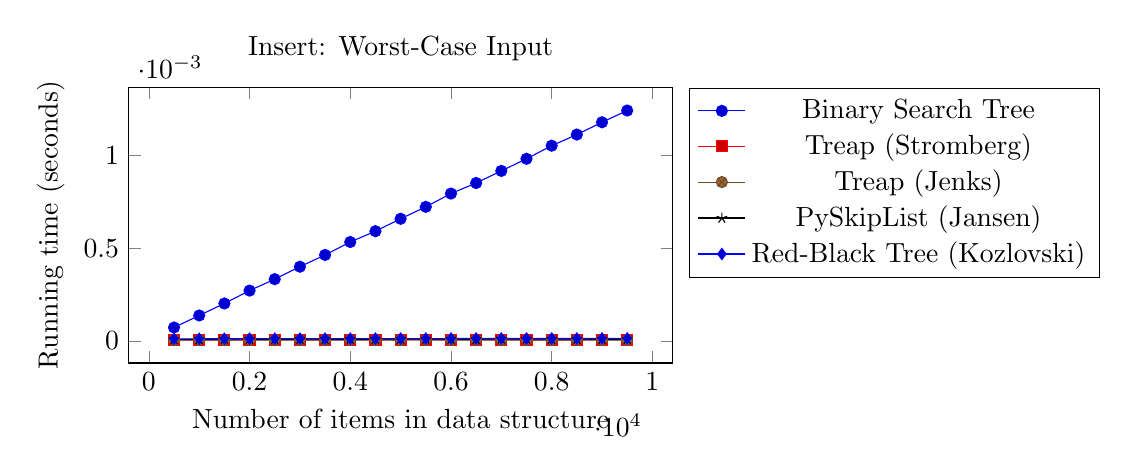
\begin{tikzpicture}
        \begin{axis}[
            xlabel={Number of items in data structure},
            ylabel={Running time (seconds)},
            title={Insert: Worst-Case Input},
            width=0.7\textwidth,
            height=2in,
            legend pos=outer north east
        ]
		\addplot coordinates {
			(500, 7.212245789192323e-05)
			(1000, 0.00013702875471527625)
			(1500, 0.000201763381596681)
			(2000, 0.00027111201463712154)
			(2500, 0.0003329101819851965)
			(3000, 0.0004002047992289903)
			(3500, 0.00046372870125665377)
			(4000, 0.000533420674180991)
			(4500, 0.0005918276072372453)
			(5000, 0.0006587035907629501)
			(5500, 0.0007231912538682206)
			(6000, 0.0007947535256337846)
			(6500, 0.0008518051696746554)
			(7000, 0.0009171090179425212)
			(7500, 0.0009825514068652907)
			(8000, 0.001053056553198859)
			(8500, 0.001113264514768879)
			(9000, 0.0011795562181412932)
			(9500, 0.0012428813444467046)
		};
		\addplot coordinates {
			(500, 4.851934675080827e-06)
			(1000, 4.830852401482844e-06)
			(1500, 4.433300956989683e-06)
			(2000, 5.475367622160832e-06)
			(2500, 5.764495945399517e-06)
			(3000, 4.767605580795475e-06)
			(3500, 4.897110975576879e-06)
			(4000, 5.83075451952908e-06)
			(4500, 5.716307891532324e-06)
			(5000, 4.4875125175991574e-06)
			(5500, 6.101812322611977e-06)
			(6000, 5.797625232482062e-06)
			(6500, 5.866895559911711e-06)
			(7000, 5.216356832562497e-06)
			(7500, 5.0416751372495125e-06)
			(8000, 4.285725041981437e-06)
			(8500, 4.586900378740211e-06)
			(9000, 5.565720223188464e-06)
			(9500, 6.011459721548817e-06)
		};
		\addplot coordinates {
			(500, 4.231513481336435e-06)
			(1000, 4.604970898931526e-06)
			(1500, 4.189348934211523e-06)
			(2000, 4.354995369446613e-06)
			(2500, 4.629064925865123e-06)
			(3000, 4.490524270970297e-06)
			(3500, 4.586900378740211e-06)
			(4000, 4.836875908260652e-06)
			(4500, 4.731464540377317e-06)
			(5000, 4.90012272894802e-06)
			(5500, 5.104921957936881e-06)
			(6000, 4.4031834233138055e-06)
			(6500, 5.041675137213985e-06)
			(7000, 4.553771091693193e-06)
			(7500, 4.2797015352391556e-06)
			(8000, 4.61099440563828e-06)
			(8500, 4.592923885482492e-06)
			(9000, 4.351983616039945e-06)
			(9500, 4.270666275125734e-06)
		};
		\addplot coordinates {
			(500, 7.938981876804974e-06)
			(1000, 8.201004419738923e-06)
			(1500, 9.083448156417263e-06)
			(2000, 8.899731200990858e-06)
			(2500, 7.932958370062693e-06)
			(3000, 9.354505959535686e-06)
			(3500, 8.794319833143049e-06)
			(4000, 8.6708379450684e-06)
			(4500, 8.80034333988533e-06)
			(5000, 1.0029138713818498e-05)
			(5500, 9.60146973564946e-06)
			(6000, 9.294270892148404e-06)
			(6500, 8.30641578758673e-06)
			(7000, 1.0315255283757097e-05)
			(7500, 1.0294173010194641e-05)
			(8000, 9.718928116981829e-06)
			(8500, 9.459917327383493e-06)
			(9000, 8.490132743013135e-06)
			(9500, 9.047307116034632e-06)
		};
		\addplot coordinates {
			(500, 1.0550172046421835e-05)
			(1000, 1.1086264145809821e-05)
			(1500, 1.1438639289806928e-05)
			(2000, 1.1637415012089036e-05)
			(2500, 1.1851249501155791e-05)
			(3000, 1.1941602102218952e-05)
			(3500, 1.2122307304274216e-05)
			(4000, 1.213134256435211e-05)
			(4500, 1.2333130040005359e-05)
			(5000, 1.2293977246216059e-05)
			(5500, 1.2402400367435007e-05)
			(6000, 1.240842387414176e-05)
			(6500, 1.2682493430595799e-05)
			(7000, 1.2625270116650712e-05)
			(7500, 1.2673458170517903e-05)
			(8000, 1.264936414354878e-05)
			(8500, 1.3019809807808257e-05)
			(9000, 1.2998727534210275e-05)
			(9500, 1.3022821561143872e-05)
		};
        \legend{Binary Search Tree, Treap (Stromberg), Treap (Jenks), PySkipList (Jansen), Red-Black Tree (Kozlovski)}
        \end{axis}
    \end{tikzpicture}
    \caption{Average of 100 operations, benchmarked every 500, starting at 500.}
\end{figure}